\documentclass[11pt,a4paper]{article}
\input{~/Documents/latex-config/math-preamble}
\usetikzlibrary{arrows,positioning,calc}

\title{DA4005 - Homework Set 3}
\author{David Sermoneta}
\date{\today}

\begin{document}
\maketitle
\begin{assignment}
There are $n$ stones in a pile. Two players alternate moves. On a move, a player may remove $1$, $3$, or $4$ stones. The player who removes the last stone wins.
\begin{enumerate}[(a)]
\item Define a Boolean DP table deciding whether the current player has a winning strategy with $n$ stones.
\item Compute recursively the winning and losing positions for $0\leq n\leq 20$.
\end{enumerate}
\begin{proof}[Solution of (a) and (b)] 
\[
\begin{array}{c|ccccccccccccccccccccc}
 & 0 & 1 & 2 & 3 & 4 & 5 & 6 & 7 & 8 & 9 & 10 & 11 & 12 & 13 & 14 & 15 & 16 & 17 & 18 & 19 & 20 \\
\hline
 & L  & W & L & W & W & W & W & L & W & L & W  &  W & W  & W  & L  & W  & L  & W  & W  & W  & W  \\
\end{array}
\] 
Clearly being at $1$ stone gives you a winning move, and so it is a winning
position. If we go to $2$ we can only remove $1$ stone, meaning it is a losing
position. Since the current player can always choose to remove one single
stone, any losing position is immediately followed by a winning position. If
the current amount is $4$ stones, this is also a winning position because we
can just remove $4$ stones.  For $5$, it's  a winning position because by
removing $3$ stones, the opponent has $2$ stones, which is a losing position,
and for $6$ stones the current player can just remove $4$ stones and get the
same result.
 
This will now keep going, since after $4$ winning positions in a row, there
will be a sequence of winning and losing positions, until there are $4$
winning positions in a row again. Note after $4$ winning positions in a row, there
can only be a losing position, and that will also be followed (again) by a winning position. The next amount of stones is now a losing position, because the table will look like $W \quad W \quad L \quad W$, the current player can only remove an amount of stones that puts the opponent in a winning position. So this is a losing position, which then is followed by 4 winning positions in a row (by the same procedure as our base case), and so by induction we know this table holds for arbitrary many stones.
\end{proof}
\end{assignment}


\begin{assignment}
 Run Kruskal's algorithm on the connected weighted graph below; all \newline weights are distinct.
\[
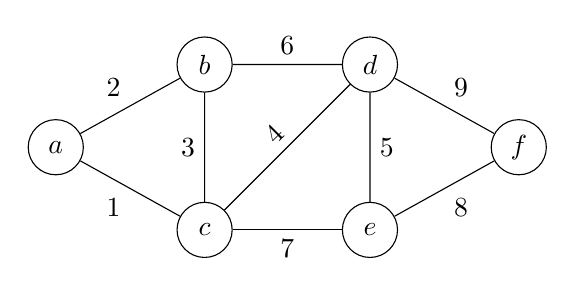
\begin{tikzpicture}[
  scale=1.05,
  vertex/.style={draw,circle,minimum size=7mm,inner sep=0pt},
  every edge/.style={thick}
]
\node[vertex] (a) at (0,1) {$a$};
\node[vertex] (b) at (1.8,2) {$b$};
\node[vertex] (c) at (1.8,0) {$c$};
\node[vertex] (d) at (3.8,2) {$d$};
\node[vertex] (e) at (3.8,0) {$e$};
\node[vertex] (f) at (5.6,1) {$f$};
\draw (a)--node[above left] {$2$}(b);
\draw (a)--node[below left] {$1$}(c);
\draw (b)--node[left] {$3$}(c);
\draw (b)--node[above] {$6$}(d);
\draw (c)--node[above,sloped] {$4$}(d);
\draw (c)--node[below] {$7$}(e);
\draw (d)--node[right] {$5$}(e);
\draw (d)--node[above right] {$9$}(f);
\draw (e)--node[below right] {$8$}(f);
\end{tikzpicture}
\]
\begin{proof}[Solution for (a)]
  First we select $ac$ and $ab$ since their selection does not
induce any cycles. $bc$ is rejected, since that would give us
the cycle $ab,bc,ac$, and so we go over to $cd$ which gets
selected, and same for $de$. $bd$ now has to get rejected
because $ab, bd, cd, ac$ would be a cycle, and we have
selected all the other ones so next is just $ef$ which we
select since no path exists to vertex $f$ yet. 
\end{proof}

\begin{proof}[Drawing]
 It's the exact same tree given by running Kruskal, since it returns the minimal spanning forest, and in our case it is just a tree. The weight of this tree is $20$. 

\[
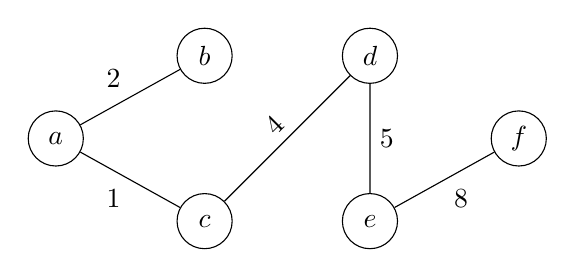
\begin{tikzpicture}[
  scale=1.05,
  vertex/.style={draw,circle,minimum size=7mm,inner sep=0pt},
  every edge/.style={thick}
]
\node[vertex] (a) at (0,1) {$a$};
\node[vertex] (b) at (1.8,2) {$b$};
\node[vertex] (c) at (1.8,0) {$c$};
\node[vertex] (d) at (3.8,2) {$d$};
\node[vertex] (e) at (3.8,0) {$e$};
\node[vertex] (f) at (5.6,1) {$f$};
\draw (a)--node[above left] {$2$}(b);
\draw (a)--node[below left] {$1$}(c);
\draw (c)--node[above,sloped] {$4$}(d);
\draw (d)--node[right] {$5$}(e);
\draw (e)--node[below right] {$8$}(f);
\end{tikzpicture}
\]
\end{proof}

\begin{proof}[Proof of (c)]
We show the statement for a connected graph $G$, since then it
will hold for the components of any graph. We will prove the
acyclic edge sets form a matroid by showing the spanning trees of $G$
form a basis. Let $T_1$ and $T_2$ be spanning trees, and $ab$ be an edge
in $T_1 \setminus T_2$, then there is a distinct path $P(a,b)$ between
$a$ and $b$ that exists in $T_2$. Removing $ab$ from $T_1$ yields us with
two components, and necessarily, an edge in $P(a,b)$ must be between two
vertices in different components, so adding that edge to $T_1 \setminus
\{ab\}$ yields us with another tree, since connecting components cannot create cycles.
\end{proof}
\end{assignment}

\end{document}
